%************************************************
\chapter{Evaluation}\label{ch:Evaluation}
%************************************************

Our evaluation considers, for simplicity, only Polybench\cite{Polybench} right now. The benchmark suite contains small isolated examples that can directly make use of static expansion to eliminate false dependencies as much as possible (Obviously, this uncovered a few bugs that need to be ironed out as well).

For the evaluation of this project, we have generated a set of patches that add compile-time statistics. These patches are not yet integrated into Polly as of now, but will be added shortly. These statistics enable us to count the number of accesses we were able to expand and would have been able to expand, if Copy-In/-Out is available. Furthermore, we track the amount of memory that is required in both situations. This gives as a nice estimate about the impact on the memory footprint, if we enable static expansion. This could also be used to implement a threshold for static expansion. A user might then specifiy an upper-bound on the memory-usage per SCoP to control the static expansion (not implemented).

The following charts are generated using \footurl{http://pygal.org/en/stable/}{Pygal} and \footurl{https://altair-viz.github.io/}{Altair}, two Python libraries to generate charts. Polybench comes with 30 benchmarks. Out of those 30, we are able to compile 22 successfully. Eight crash during compilation, we are investigating the reason for this. For the compile-time comparison we refer to the polybench’s EXTRALARGE\_ DATASET. For our run-time evaluation we had to use the biggest dataset that fit into the main-memory of the test-machine (a laptop with an Intel i7-2600 working at 3.40GHz and 32Go of RAM). This would be LARGE\_ DATASET for most benchmarks and MEDIUM\_ DATASET for a few selected ones. Evaluation were run using the Benchbuild suite\cite{Benchbuild}.

\section{What if copy-in/out would have been available ?}
The idea is to know, for all users of the ScopArrayInfo, if the user is inside or outside the loop in which the write (for MemoryKind::Array and MemoryKind::Value) or the read (for MemoryKind::PHI) happened.

To proove the necessity of copy-in/out implementation, we compare the number of expandable memory accesses that are expanded now and the one that would be expandable if we would have copy-in/out.

\begin{figure}
\centering
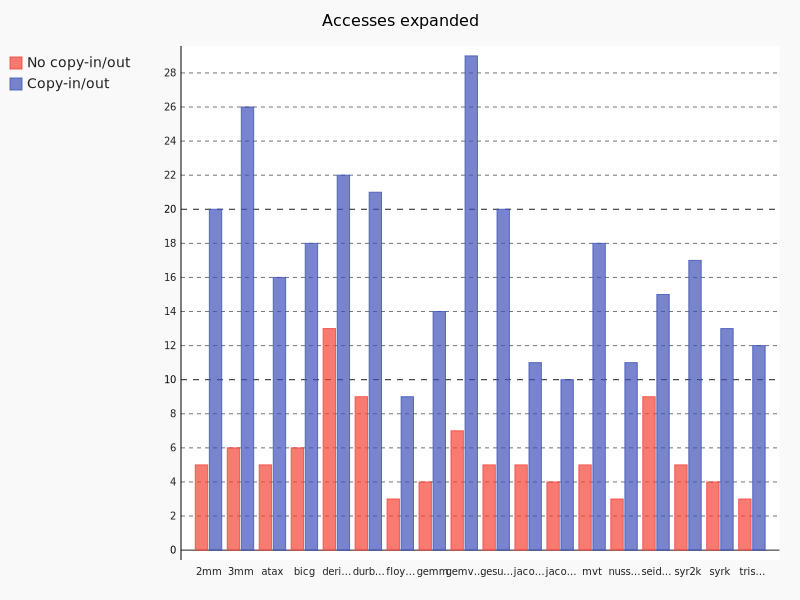
\includegraphics[scale=0.4]{gfx/Evaluation/Numbers.png}
\caption{Number of memory accesses expanded}
\label{fig:Numbers}
\end{figure}

We clearly see with Figure~\ref{fig:Numbers} that, if the copy-in/out would have been implemented, way more memory accesses would have been expanded. But expanding more memory accesses can lead to memory space problems. Let us look at the impact of static expansion on the memory needed to store the expanded arrays.

\section{Memory usage}
Obviously, static expansion can increase the memory usage quite a lot. What sounds bad at first, is actually a success for us. Because an increase in memory usage shows that we actually expanded accesses. At the same time we trade this memory for the elimination of dependencies, which in turn enables parallelization. Again, for both Copy-In/-Out available and not available we compare the memory usage for the expansion. Results are shown in Figure~\ref{fig:MemorySpace}.

\begin{figure}
\centering
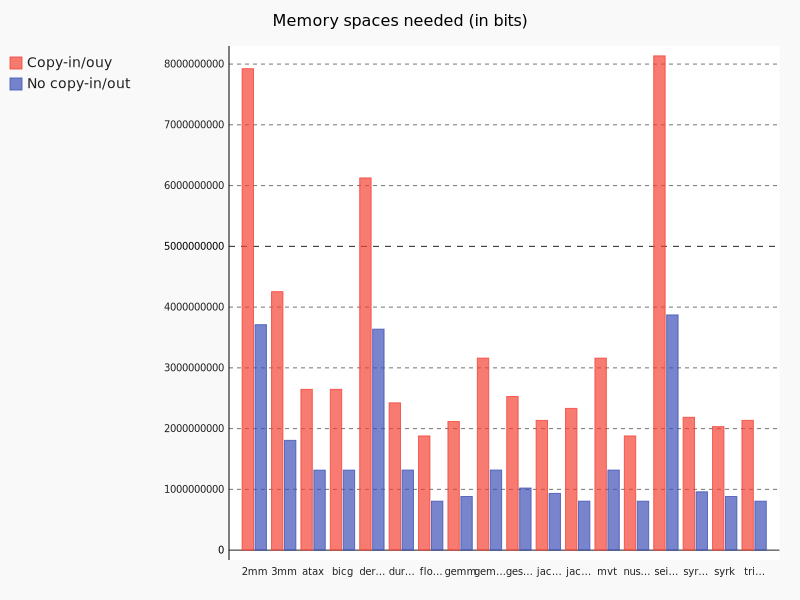
\includegraphics[scale=0.4]{gfx/Evaluation/MemorySpace.png}
\caption{Memory Space needed for expansion}
\label{fig:MemorySpace}
\end{figure}

The memory needed for array allocation is huge. For example, for 2mm without copy-in/out, with the EXTRALARGE\_ DATASET of polybench, we need more than 327Mb. If copy-in/out would have been in place, the ammount of space needed would be very large. Even if the current memory available on machines is huge, the need of a way to select which SAI to expand and also a way to expand in an efficient manner (Maximal Static Expansion) is felt.

\section{Run-time evaluation}
We close up the evaluation with an overview over the execution behavior of our static expansion implementation. At first, we look at the overall increase in memory consumption, measured with UNIX’s implementation of /usr/bin/time. This gives us access to the maximum resident size (RSS). Without any filtering we see a comparison between the baseline (-O3) and clang with static expansion enabled (MSE) enabled. For these experiments, we explicitly disabled operand-tree optimizaion and DeLICM to get an isolated view on only our transformation.

\begin{figure}
\centering
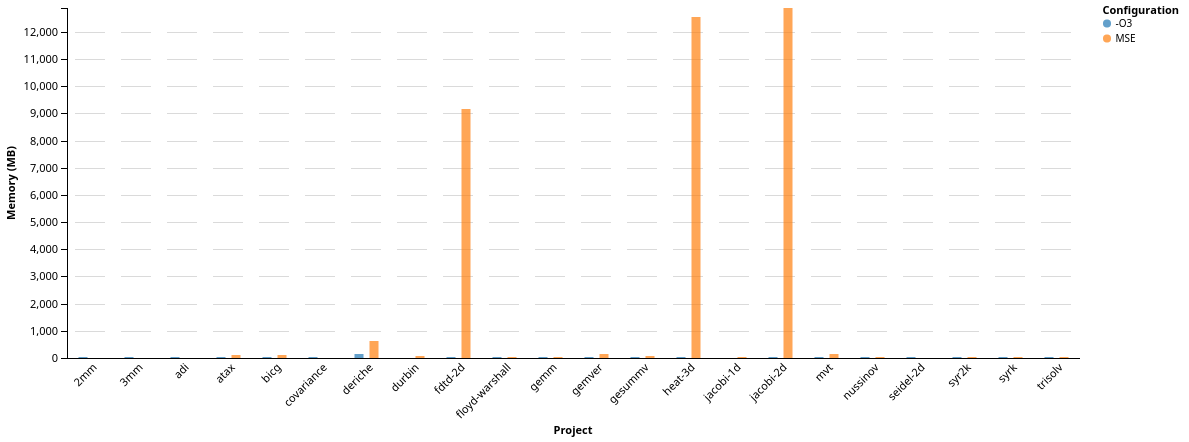
\includegraphics[angle=90,origin=c,scale=0.5]{gfx/Evaluation/RT-1.png}
\caption{Increase in memory consumption}
\label{fig:RT-1}
\end{figure}

On Figure~\ref{fig:RT-1}, we can directly see the extreme increase in memory consumption when looking at the benchmarks ‘fdtd-2d’, ‘heat-3d’, ‘jacobi-2d’. If we look at memory consumption values lower than 200MB, we can get a more detailed view on the remaining benchmarks (see Figure~\ref{fig:RT-2}).

\begin{figure}
\centering
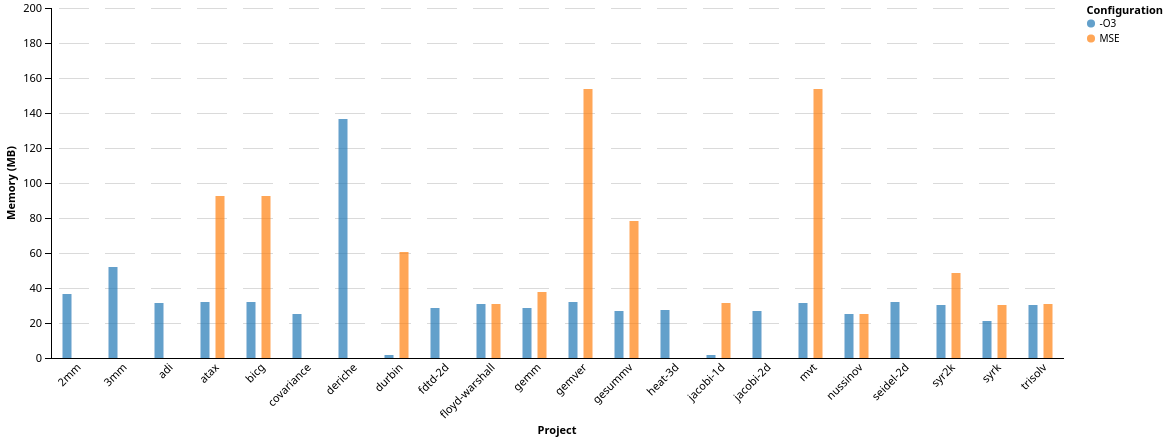
\includegraphics[angle=90,origin=c,scale=0.5]{gfx/Evaluation/RT-2.png}
\caption{Increase in memory consumption on a subset of Polybench}
\label{fig:RT-2}
\end{figure}

As expected, whenever we are able to expand accesses, we increase the amount of memory consumed by the benchmark. We also can see the benchmarks where we were not able to finish compilation/execution, either because of bugs in our code, or due to being killed by the systems OOM-Killer process (we reserved too much memory for the system to handle). Finally, without any schedule optimization enabled in Polly, we did not expect to be able to gain speedup by just expanding memory accesses. However, due to the reduction in dependencies, we already enable transformations in the Polly optimization pipeline, e.g., tiling.

\begin{figure}
\centering
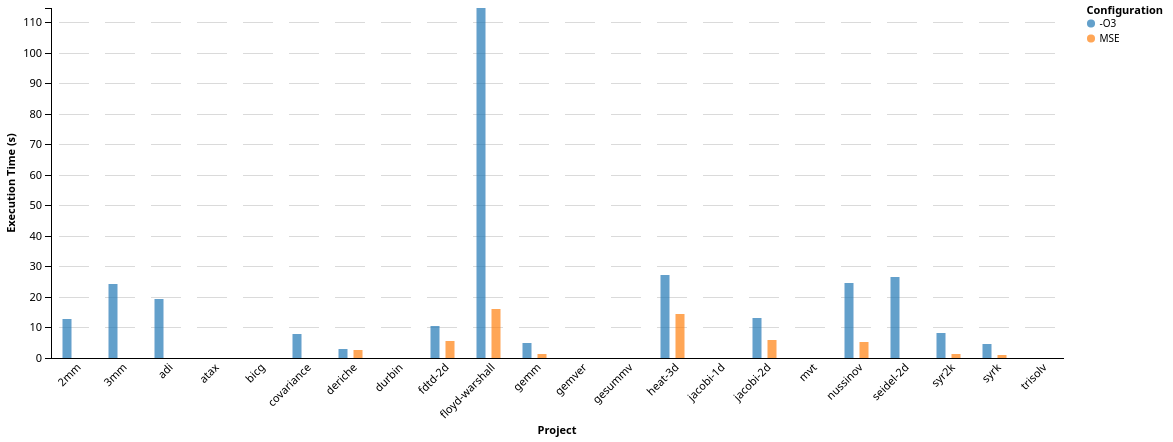
\includegraphics[angle=90,origin=c,scale=0.5]{gfx/Evaluation/RT-3.png}
\caption{Comparison of execution time with and without \ac{FIE}}
\label{fig:RT-3}
\end{figure}

Interestingly, we can see on Figure~\ref{fig:RT-3} that the benchmarks ‘floyd-warshal’, ‘nussinov’, did not suffer from memory consumption increase, although we were able to expand accesses at compile-time. This suggests that by expanding an already fully-dimensional access we were able to change the memory access pattern in a positive way. A missing orange bar means that the benchmark crashed at run-time either because of a bug in our expansion, or because of too much memory being consumed. These will be resolved in the next weeks.
